% ---------------------------------------------------- %
% Budburst 2015 manuscript
% Preamble
% ---------------------------------------------------- %
\documentclass[11pt]{article}
\usepackage{textcomp}
\usepackage{fontenc}
\usepackage{graphicx}
\usepackage{caption} % for figure captions
\usepackage{gensymb} % for \degree
\usepackage{placeins} % for \images
\usepackage[margin=1in]{geometry} % to set margins
\usepackage{setspace}
\usepackage{lineno}
\usepackage{cite}

\doublespacing
\renewcommand{\familydefault}{\sfdefault} % for nicer sans serif font
\graphicspath{{images/}}	% Root directory of the figures
\setlength{\parskip}{2 mm}

\usepackage{Sweave}
\begin{document}

\linenumbers
\Sconcordance{concordance:Budburst.tex:Budburst.Rnw:%
1 21 1 1 0 146 1 1 7 1 1 1 11 16 0 1 3 1 14 26 0 1 2 2 1 1 4 15 0 1 4 %
15 0 1 4 15 0 1 4 15 0 1 3 29 1}
 

\flushleft
\textbf{\large{Photoperiod and temperature interactively drive spring phenology in multiple species}}

Flynn, Wolkovich

\textit{The Arnold Arboretum of Harvard University}
%%%%%%%%%%%%%%%%%%%%%%%%%%%%%%%%%%%%
% Abstract
%%%%%%%%%%%%%%%%%%%%%%%%%%%%%%%%%%%%
% First two sentences are good -- but you only have room for one 'why to care about phenology' statement so adjust. - dropped first one
% Also need a quicker intro to design, including a clear problem statement. Consider something along the lines of: how diverse species respond to warming is a big question but few studies have looked at many species and such work has been generally observational. - added to 2nd paragraph
% Observational studies, however, have known difficulties in teasing out plant responses to climate with are generally thought to be based on one or several major cues plant receive from the fall to spring: chilling temperatures, photoperiod and spring forcing temperatures. For a handful of well-studied temperate woody species these cues appear to be interactive, meaning predictions of plant responses to climate change will be complex and non-linear (cite CHUINE). Other work, however has suggested many species may be dominated by one of the three possible cues (cite Korner & Basler), making some species responses simple to predict. - added to 1st paragraph

\textbf{Understanding the sensitivity of forest plants at the species level to abiotic drivers of plant phenology is critical for developing predictions of community composition, changes in community composition resulting from climate change, and resulting alterations to ecosystem-level properties such as carbon sequestration.  While observational studies of long-term trends are essential for understanding how climate affects timing of phenological events, experimental manipulations are necessary to disentangle otherwise covarying environmental factors and directly assess species- and individual-level responses to climate change factors. Observational studies have additionally known difficulties in teasing out plant responses to climate, with responses expected to be based on one or several major cues plant receive from the fall to spring: chilling temperatures, photoperiod and spring forcing temperatures. For a handful of well-studied temperate woody species these cues appear to be interactive, meaning predictions of plant responses to climate change will be complex and non-linear \cite{Chuine:1999aa}. Other work however has suggested many species may be dominated by one of the three possible cues \cite{Korner:2010}, with a tradeoff between photoperiod and forcing temperature sensitivities, making some species responses simple to predict. However, range of responses across species within a forest community to winter chilling temperatures, photoperiod, and spring forcing temperatures have received relatively limited attention. Given the wide range of budburst and leaf out across temperate woody species \cite{Polgar:2011aa}, these species differences may be crucial in scaling up to ecosystem-level responses. Here we present results from an experimental manipulation of spring forcing temperatures, photoperiod, and intensity of winter chilling with dormant clippings of 28 woody plant species from forest communities at two latitudes (42.5\degree N and 46\degree N). We show photoperiod sensitivity is common across northeastern woody plants and phenological sensitivity to photoperiod and temperature appears largely coordinated across species (i.e., species highly sensitive to temperature were also highly sensitive to photoperiod), with greater sensitivity of budburst and leaf out to temperature than to photoperiod. Winter chilling exerts a large role in driving advances in spring phenology, for both budburst and leaf out stages, yet more intense chilling at 1.5\degree C resulted in less pronounced effects than at 4\degree C. Latitude of origin exerted surprisingly small effects on sensitivity to abiotic factors in driving spring phenology, indicating that local adaptation---at least across 4\degree of latitude---may not necessarily constrain woody plant responses to climate change. Shrub and small tree species were less sensitive to changing temperatures or photoperiod, but consistently earlier in their phenology. These results indicate that under warming conditions, communities could shift to a more canopy-tree dominated system with generally later phenologies, counteracting advances in phenology at the ecosystem scale.}

%%%%%%%%%%%%%%%%%%%%%%%%%%%%%%%%%%%%
%Introduction 
%%%%%%%%%%%%%%%%%%%%%%%%%%%%%%%%%%%%

Woody plant spring phenology drives global carbon cycles and local ecosystem properties, from the length of the growing season to energy balance between land and atmosphere. Timing of spring phenology in temperatue woody plants is critical for understanding net ecosystem assimilation at the forest scale, as maximizing the length of the growing season and minimizing risk of tissue loss due to early spring freezing depends on accurate timing of budburst and leaf out \cite{Basler:2014aa}. The crucial role that phenology plays in these ecosystem processes, and the indications that plant and animal phenology are advancing as rapidly as 2.3\degree C per decade \cite{Menzel:2006} have led to increased attention to tracking the patterns of phenology at large temporal scales. Observational studies of long-term trends are crucial for understanding how climate affects timing of such phenological events, and in combination with field and growth chamber studies, it is clear that spring phenology for woody plants in temperate ecosystems is driven by a combination of increasing spring temperature (forcing), length and intensity of winter temperature (chilling), and changing daylength (photoperiod). Observational studies generally show stronger signs of phenological advance in response to temperature than experimental manipulations \cite{Wolkovich:2012aa}, yet experimental manipulations are necessary for disentangling otherwise covarying environmental factors and directly assess species- and individual-level responses to climate change factors. 

% Plant strategies and risk
% Hypotheses for plant strategies: 
% 1. freezing tolerance (go early) vs freezing avoidance (go late)
% 2. opportunistic/risky (go with temperature) vs conservative (go with photoperiod and chilling)

% early, not going with temperature: tolerance. This is what we find for the shrubs!
% late, going with temperature: avoidance but opportunistic: this is what we find for the trees. 

% This might also be a way to sneak in the traits possibly ... because I think the strategy could be early, risky but cheaper, less competitively dominant versus later, safer and more competitively dominant. Then the traits work provides a very simple test of this? And we say 'ah, teasing out the traits will be trickier and probably involve understanding which traits really tie to competitive superiority versus which might tie to frost resistance etc.. 
Adaptive pressues drive temperate woody plants to balance the maximization of carbon gain with minimzation of freezing risk in spring phenology. 

Spring frost events have been increasing in North America \cite{Augspurger:2013aa}, with greater probability of freezing events occuring after budburst. A single frost event, if timed after leaf out, can substantial reduce ecosystem productivity \cite{Gu:2008aa} and potentially shift the composition of temperate forests \cite{Hufkens:2012aa}. 

Plants may either tolerate risk of spring freezing by investing in tissue which can withstand freezing, or avoid freezing with later phenology. For perennial plants, it has been found that leaves of species which have later phenologies can be more sensitive to frost damage \cite{CaraDonna:2014aa}\cite{Vitasse:2014aa}, supporting the notion of a tradeoff between tolerance and avoidance of freezing risk. Avoidance should be an adaptive strategy when the risks of freezing damage is high and damage severe enough to make the benefits of early spring phenology not worth the cost of tissue loss \cite{Sakai:1987aa}. Physiologcially, tolerance to freezing is driven by resistance to rupturing of biomembranes, and is related to dehydration stress \cite{Larcher:2005aa}. Plant functional traits related to freezing resistance thus are likely to include high tissue density, both of leaves and stems. Avoidance-strategy plants would be expected to express lower tissue densities, with the shorter growing season being made up for by faster growth rates, less investment in structural elements of tissue, and relatively greater percent nitrogen in leaves. 

The other key tradeoff that can be expected is between opportunistic plant strategies, where temperature is the dominant driver of spring phenology, and conservative strategies, where photoperiod and chilling are the key drivers. Opportunistic strategies should benefit species in a non-stationary environment, as in a warming world where mild winters are less an unusual occurance. It has been stated that short-lived, early successional species typically exhibit such opportunistic strategies, and late-successional species are more typically photoperiod-controlled \cite{Korner:2010}, yet multi-species tests of this proposal have not been carried out. As the abiotic environment is hardly the sole contributor to plant performance, considering a suite of co-occuring species together is key for making progress in understanding the role phenology plays in shifts in community composition and ecosystem functioning. 

% Latitude
The role of latitude in how abiotic drivers determing spring phenology has largely been investigated in single-species studies across many sites. Given sufficent distance, more pole-ward sites have lower minimum annual temperatures and shorter growing seasons, making accurate timing of spring phenology even more important. Since daylength differences from winter to spring are also greater for higher latutitudes, populations of northern plants may be expected to rely more on photoperiod as a cue for spring phenology.

For temperate trees, species can be limited at their northern range by inability to develop mature fruit in a given growing season, while limited at their southern range by inability to break dormancy due to insufficient chilling \cite{Chuine:2010}. Thus phenology can drive range limits. Common garden studies have shown that southern-adapted species, when translocated to a more northern location, exhibit later leaf out compared to species adapted to northern sites \cite{Zohner:2014aa}. If species remain relatively fixed in their timing of leaf out, then northward migration of such late-phenology species may act to counteract community-wide advances in phenology under a warming climate. 

% photoperiod
Photoperiod has long been known to be a critical driver of the onset of endormancy, in combination with cooling temperatures \cite{Foley:2009aa}. However, the role of photoperiod in determining the breadking of dormancy has been debated, with various authors finding that the strength of daylength as a driver may depend on phenological stage, species and location \cite{Heide:1993}\cite{Falusi:1996aa}. Photoperiod and winter chilling can interact, as long photoperiod enhances cell growth, compensating for a lack of chilling during the endodormancy phase \cite{Heide:1993b}\cite{Caffarra:2011aa}\cite{Myking:1995}. In the few experimental studies that have directly manipulated both forcing temperature and photoperiod, photoperiod has been shown to act to moderate advances in phenology due to warming, with reduced advances due to temperature when daylength was short \cite{Sanz-Perez:2009aa}\cite{Heide:1993b}. 
% look for additional refs showing non-additive effects (replacability)

% Chilling
% points to make: chilling is a strategy to make sure budburst/leaf out do not occur too early. This can be a supplemental stragety in addition to photoperiod and temperature cues for breaking endodormancy. [notes to myself: endodormancy: short days in fall. Broken by chilling. Ecodormancy: broken by temperature.

In addition to photoperiod, winter chilling requirements also act as a conservative strategy to avoid damage from early spring freezing, allowing woody plants to avoid breaking bud during unusually early warm spells \cite{Ghelardini:2010aa}. To an extent, these three factors of temperature, photoperiod, and chilling are interchangeable, such that plants experiencing mild winter with insufficient chilling can still break bud given sufficiently long photoperiods and warm temperatures \cite{Heide:1993b}. Chilling requirements are known to vary substantially across species, with some needing relatively little winter chilling to initiate budburst, and others not bursting bud even in long-day, warm envronments unless sufficient chilling has taken place \cite{Korner:2010}. 

% Why do cuttings: can manipulate abiotic conditions on same individual, species specific, can detect early events with more precision than larger-scale studies

Knowing species-specific sensitivies of temperate plant phenology to chilling and forcing alone can predict regional-scale phenology \cite{Chuine:2000}. Substantial variation exists at the species level in the magnitude of the temporal advance of spring phenology \cite{Primack:2009aa}, such that the presence of species highly sensitive to temperature change can strongly drive community-level phenology \cite{Diez:2012}.

Early phenological events, such as initial swelling of buds and budburst (separtion of budscales) are challenging to study from remote sensing, with little obvious change in color or reflectance. 
requiring experimental work at the individual level. 
Different phenological stages may be driven by different environmental cues. The period between budburst and leaf out is critical for leaf development, as this is a period when plants are highly sensitive to damage from late freezing events, with freezing resistance increasing as leaves expand \cite{Sakai:1987aa}.

To test the interactive effects of the three controlling drivers of spring phenology, temperature, photoperiod, and chilling across latitudes, we carried out a study of 28 woody plants. We assessed both budburst and leafout to account for the potential different sensitivies of these phenological stages to abiotic drivers, and analyzed responses across all species to examine  

%%%%%%%%%%%%%%%%%%%%%%%%%%%%%%%%%%%%
\section*{Results}
%%%%%%%%%%%%%%%%%%%%%%%%%%%%%%%%%%%%

Temperature and photoperiod individually and interactively determined timing of leaf-out, with the strongest effects of temperature in short-day conditions. We found photoperiod sensitivity was common and strong across all of the woody plants studies, consistently reducing time to phenological responses for each species, across sites of origin. 

For the 28 species studied, sensitivity to temperature and photoperiod cues for leaf-out times varied substantially, and---in contrast to our hypotheses [that we set up in the intro]---co-varied overall. The coordinated response to warming temperatures and longer photoperiod was consistent with overall pace of phenological events; earlier-leafing out species (namely the shrubs \emph{Spiraea alba}, \emph{Viburnum cassanoides}, and \emph{Vaccinium myrtilloides}) exhibited relatively limited advances to either warming or longer days, while later leafing-out species showed ability to advance their phenology by in response to both warming and longer days. Thus, no trade-off was observed between photoperiod-cued and temperature-cued species, but rather species exhibit coordinated responses to both environmental factors (Fig. 1). Of the other species, \emph{Fagus grandifolia} exhibits relatively limited response to warming but substantial photoperiod sensitivity, while \emph{Rhamnus frangula} shows relatively limited response to photoperiod but substantial warming sensitivity; if only a small subset of species including these two had been included in the study, it might have been concluded that a tradeoff between photoperiod sensitivity and warming sensitivity would exist. 

While both photoperiod and temperature cues were important for driving woody plant phenology, responses to chilling were also substantial. Budburst day was accelerated most by the chilling treatments. Tables 1 and 2 summarizes hierarchical mixed-effects model analysis of day of budburst and leaf-out, with negative values indicate earlier day of experiment for each event. Overall the 5\degree C experimental warming resulted in 6.8 days earlier budburst and 21.9 days earlier leaf out. Such advance was delayed by the each chilling treatment, as indicated by the positive coefficient for the temperature x chilling interactions. Latitude of origin (Site) overall had little direct effect on budburst or leaf-out, but populations from the northern site tended to exhibit slower budburst and leaf-out, with a more rapid budburst and leaf out in response to the chilling treatments (indicated by negative coefficients for site x chilling treatments).

Warming, photoperiod, and chilling individually and interactively acted to drive budburst and leaf out earlier across species. The strength of the acceleration in budburst due to both warming and photoperiod were similar, but the acceleration of leaf out due to warming exceeded that of photoperiod for both phenological stages. Surprisingly, site of origin exerted limited effect on either budburst or leaf out across species. 

\subsection*{Effect of chilling}
The cuttings were harvested in late January 2015, and thus experienced substantial natural chilling by the time they were harvested. Using weather station data from the Harvard Forest and St. Hippolyte site, chilling hours (below 7.2\degree C), Utah Model chill portions (hours below 7.2\degree C and between 0\degree C and 7.2\degree C) and Dynamic Model \cite{Erez:1988} chill portions were calculated both for the natural chilling experienced by harvest and the chilling experienced in the 4\degree C and 1.5\degree C treatments. The Utah Model and Dynamic Model of chill portions account for variation in the amount of chilling accumulated at different temperatures, with the greatest chilling occurring approximately between 5-10\degree C, and fewer chill portions accumulating at low temperatures and that higher temperatures can reduce accumulated chilling effects. The two differ in the parameters used to determine the shape of the chilling accumulation curve, with the Dynamic Model being shown to be the most successful in predicting phenology for some woody species \cite{Luedeling:2009}.
With both the Utah and Dynamic model, the more severe chilling treatment resulted in fewer calculated chilling portions. 
% Need to describe each model super briefly! - done

Species varied widely in response to chilling treatments, with some exhibiting strong chilling requirements (\emph{Acer saccharum}, \emph{Fagus grandifolia}), while others exhibited little change in phenological advancement under experimentally manipulated chilling. Overall, budburst and leaf-out advanced by 22.1 or 26.4 days under additional 30 d of vernalization at 4\degree C, and advanced by a reduced amount of 19.7 or 26.1 days under 30 d of vernalization at 1.5\degree C. The reduced chilling effect at the lower temperature chilling is consistent with the Dynamic Model of chilling accumulation. % And also consistent with the Utah model?

Species-specific responses to chilling demonstrate that chilling requirements are not uniform across species, with 
of \emph{Fagus grandifolia} to increasingly strong vernalization varies by latitude of origin and by phenological stage; winter chilling reduced day to budburst and leaf-out, but more strongly for individuals from the northern site.

While nearly all species showed advances in spring phenology in response to the experimental chilling treatment, as indicated by fewer days to phenological events for the 4\degree C and 1.5\degree C treatments, the majority of species (e.g. \emph{Populus grandidentata}) showed delays in both budburst and leaf out at the more severe chilling treatment. Of the species exposed to the additional chilling, only \emph{Fagus grandifolia} was consistently advanced by the more severe chilling.

\subsection*{Species-specific responses}

Species traits partly explain variation in warming and photoperiod sensitivities of leaf out. Plants with high nitrogen leaves, as well as high SLA (thinner, less dense) leaves, were significantly later in both budburst and leaf out. Thus early leaf out species tended to be tougher, less N-dense, and have higher carbon investments than later species. Greater wood density had inconsistent effects as a driver, with higher wood density driving later budburst but tending to drive earlier leaf out.

Ring-porous species (\emph{Fraxinus sp.}, \emph{Lonicera}, \emph{Myrica}, and \emph{Quercus}; lower values of Pore Anatomy variable) exhibited significantly later budburst and leaf out compared to diffuse-porous species, in line with previous work on wood anatomy and freezing risk \cite{Sperry:1992}.

Shrubs with low specific leaf area (thick/dense leaves) and high stem density were more likely to leaf out earlier. For trees, with an overall later leaf out pattern, 

Rank order of leaf out and budburst was stable across warming and photoperiod treatments. Chilling treatments shifted the order, for example \emph{Fagus grandifolia} was the 23-28th species to burst bud with no additional chilling, but advanced to the 10-11th species to burst bud in with additional chilling. Within chilling treatments, the consistency of the rank order was high, with standard deviation of the rank order ranging from 2.05 d (budburst, no additional chilling) to 0.75 d (leaf out, additional chilling at 4\degree C). Compared to field observations, rank order of leaf out was generally most related in the cool, short-day treatment with no additional chilling (Fig. S10).

\subsection*{Nonleaf outs}

Across all treatments, 20.2\% of the cuttings did not break bud or leaf out. Across species, there was no overall predictive effect of temperature, photoperiod, chilling, or site on the propensity to fail to leaf out. Species ranged from complete leaf out (\emph{Hamamaelis}) to only 50\% leaf out (\emph{Fagus grandifolia}, \emph{Acer saccharum}) across all treatments. The percent of nonleaf outs by site was similar, with 20.6\% of Harvard Forest and 19.7\% of St. Hippolyte samples failing to leaf out. Examining individual species,  there was an interaction of temperature by day length for selected species, with greater failure to leaf out in cool, short-day conditions for \emph{Acer pensylvanicum}  and \emph{Acer saccharum}. Site effects were inconsistent, with greater failure to leaf out for cuttings from St. Hippolyte in \emph{Acer rubrum} and \emph{Fagus grandifolia}, and from Harvard Forest in \emph{Acer saccharum}. 

% I think you can cut the below
% All species show advances in budburst and leaf out in response to photoperiod, warming, and chilling treatments. All species showed positive interactions between warming and chilling for leaf out. For budburst, interactions between warming and chilling were always positive but not those between photoperiod and chilling (4 and 12 species showing positive interaction for chill1 and chill2, respectively).


%%%%%%%%%%%%%%%%%%%%%%%%%%%%%%%%%%%%
\section*{Discussion}
%%%%%%%%%%%%%%%%%%%%%%%%%%%%%%%%%%%%

Photoperiod sensitivity is common in northeastern woody plants, and greater photoperiod sensitivity is related to, not instead of, temperature sensitivity. Taken together, this result shows that the opportunism-conservatism tradeoff is not supported by the data for this suite of species. The most sensitive species to both cues, namely the species which could advance their phenology in response to both longer days and warmer temperatures, were the later-successional tree species, rather than the shrubs. The trait data indicate partially that the species earliest to leaf out, namely the shrubs and small trees, also had lower SLA and lower leaf \%N, indicating greater investment in tissue structures. These results support the tolerance-avoidance tradeoff, with the early phenology species being tolerant to freezing but relatively less able to advance their phenology in a warming environment. These results also indicate that the later-successional species have potentially the most to gain from a warming world, as they can extend their growing seasons  

While both photoperiod and temperature sensitives were common, chilling sensitivity greatly outweighed both of these factors. It is important to note that the results from the chilling part of this experiment are derived from 11, not 28 species, but the strength of this effect is notable. Strong chilling requirements were detected both for budburst and leaf out responses, and the most substantial advance in spring phenology came from the more mild chilling treatment, at 4\degree C, with reduced effectiveness of chilling at 1.5\degree C. 

These three factors did show some degree of substituability, meaning for example that a lack of chilling could be made up for by an increase in temperature. These are indicated by the positive two-way interactions; chilling and forcing temperature are more substitutable than chilling and photoperiod, for both budburst and leaf out.

We found only limited support for the northern populations showing more conservative (photoperiod-cued) strategies in these 28 species was found, with small delays in both phenological events for populations from the more northern site. The latitudinal range studied here is within the range of the phenotypic flexibility of these species. Of these study species, we should not be overly concerned about being photoperiod limited at the more northern sites; given sufficient pace of dispersal, they will be able to track a changing climate.

Budburst is sensitive to the same environmental cues as leaf out, but species show idiosyncratic orderings of their sensitivity to environmental cues at these two phenological stages; leaf out responses can not necessarily be used to back-cast budburst responses. Budburst showed a more limited total response to environmental cues, and species were more tightly clustered in those responses.

Surprisingly, the smaller statured, earlier-leafing out shrubs and small trees exhibited reduced sensitivity to all three factors of temperature, photoperiod, and chilling. They are relatively more fixed in their timing of both budburst and leaf out, perhaps indicating an alternative mechanism for timing of spring phenology in these plants \cite{Pagter:2015}.

Given these results, the future of the northeastern forests may shift towards later-phenology, canopy trees, as these species demonstrated a greater ability to lengthen their growing seasons opportunistically in response to warmer temperatures.
% I think we should be more cautious in stating this. We still don't know *what* controls their leaf out! -- I think we can make some educated guesses here!

% Re the above about shrubs versus trees -- I am just not sure what to think! And it comes back to the models. Our models give each species a fundamental leaf out day -- their intercept. This makes lots of sense to me but biologically I am not sure what to do with it (and if we take it away then the early species become hyper-sensitive, right? - right). I think we need to think on what that intercept means and what we should and shouldn't say given that it's in our models. I think it could be what you suggested, it could also be that they have super weak chilling, it could be that they are sensitive to humidity or something we don't study. But fundamentally I think we need to think harder about that before we push our conclusions too far. 
%%%%%%%%%%%%%%%%%%%%%%%%%%%%%%%%%%%%
\section*{Methods}
%%%%%%%%%%%%%%%%%%%%%%%%%%%%%%%%%%%%
\textbf{Field sampling}

Woody plant cuttings were made in January 2015 for 28 species which occurred in both Harvard Forest (HF, 42.5\degree N, 72.2\degree W) and the Station de Biologie des Laurentides in St-Hippolyte, Quebec (SH, 45.9\degree N, 74.0\degree W). The typical late January temperatures are -3.4 and -22\degree C, respectively; day length between these two sites differs by a maximum of 45 minutes. Weather station data from each field site was obtained for calculations of chilling units. 

Species were chosen based on the dominant forest vegetation at each site, aiming to maximize the number of shared species between the two sites. Of the 28 species, 19 occurred at both sites. Comparing only shared species, the mean days to budburst and leaf out across all treatments for Harvard Forest and St. Hippolyte was 25.6/36.8 and 24.8/36.1 days, respectively (Table S1). For each species, up to 15 representative healthy, mature individuals with branches accessible by pole pruners from the ground were tagged in late summer and fall 2014. In winter 2015, six individuals were located and 4-16 cuttings taken from each individual, depending on size of the individual and number of treatments to be applied. Cuttings were kept cold and transported back to the Arnold Arboretum in Boston, MA.
%The species chosen represent XXX percent of the basal area in Harvard Forest and St. Hippolyte, respectively.

\textbf{Growth Chamber Study}

Cuttings were placed in growth chambers at the Arnold Arboretum in Erlenmeyer flasks distilled water, with water changed every 7-10 days. The base of cuttings was re-cut at each water change under water to prevent callusing. For 11 of the 28 species, sufficient cuttings were obtained from each individual tree to apply the full set of 12 experimental treatments: 2 temperature (20\degree C / 10\degree C warm vs. 15\degree C / 5\degree C cool) x 2 photoperiod (12 vs. 8 h) x 3 chilling (no additional chilling,  additional 33 d at 4\degree C, or 33 d at 1.5\degree C) treatments. For the remaining 17 species, only sufficient cuttings were obtained to apply the temperature and photoperiod treatments, without the additional chilling levels. The total number of cuttings for a given species thus ranged from 24 to 144, depending on presence at each site and application of the chilling treatment.

Phenology of the cuttings was assessed using a modified BBCH scale \cite{Finn:2007}, with observations on each of the 2,136 cuttings made every 2-3 days for the course of the 82-day experiment, a total of 48 observation days. The phenological stages assessed in the present study are budburst, defined as beginning of sprouting or bud breaking or shoot emergence (Code 07 in \cite{Finn:2007}) and leaf out, defined as first leaves unfolded (Code 11 in \cite{Finn:2007}). Additional stages up to flowering and stem elongation were also recorded. In total, we made 19,318 phenological observations at the cutting level.

\textbf{Functional trait collection}
In summer 2015, the same individuals previously tagged in the field were revisited as part of an additional study. Six individuals of each species were sampled for several plant functional traits, following standard protocols \cite{Perez-Harguindeguy:2013aa}. In some cases, the individual used in the growth chamber study was missing, in poor condition, or had no remaining branches to sample, and was replaced by a nearby representative individual. For each individual, height and diameter at breast height (DBH) were recorded, and leaf and stem material were sampled from the middle of the canopy or the greatest height reachable with pole pruners. Leaf material was kept cool and moist, and within several hours was scanned for leaf area and weighed fresh. Stem volume was measured using a water-displacement method. Samples were oven dried at 70\degree C and weighed within several days of sampling, and specific leaf area (SLA) were calculated stem density. Leaf tissue was further processed for carbon:nitrogen ratio using an elemental analyzer (Perkin-Elmer Elemental Analyzer) at Harvard Forest. Since in not all cases the same individual used for the growth chamber experiments was the individual sampled for functional traits.

\textbf{Statistical analysis}

For the two phenology responses measured, we fit mixed effect models separately for day of year, using site, warming, photoperiod, and chilling treatments as predictors and species as a modeled groups (random effects). For each model, two-way interactions for effects of site, warming, and each of the chilling treatments were included. Simplified versions of models were initially fit using the \emph{lme4} package in the statistical programming environment \texttt{R}, then full versions of the model were fit using a Markov Chain Monte Carlo sampling approach in the programming language \texttt{Stan} (\texttt{www.mc-stan.org}).

% Add? "fit using a Baeysian approach with weak priors"...
% add: Bob Carpenter, Andrew Gelman, Matt Hoffman, Daniel Lee, Ben Goodrich, Michael Betancourt, Michael A. Brubaker, Jiqiang Guo, Peter Li, and Allen Riddell. 2016. Stan: A probabilistic programming language. Journal of Statistical Software (in press).

\textbf{Phylogenetic methods}

We tested the influenced of phylogenetic relatedness on the relationship between functional traits and sensitivities to warming, photoperiod, and chilling treatment. Sensitivities were extracted as the slopes of the species-level responses of leaf out day to each of the experimental factors; more negative values indicate greater advance in leaf out in response to that factor. Using a phylogenetic tree resolved at the genus level from Phylomatic (\texttt{www.phylodiversity.net}), and the \emph{caper} package in \texttt{R}, we fit phylogenetic generalized linear models between the sensitivities at the species level to the functional traits of stem density, SLA, and percent leaf nitrogen (\%N). In this type of model, the parameter $\lambda$ represents the strength of the phylogenetic symbol, with values close to 1 indicating that closely related species have more similar responses to the abiotic drivers.

%%%%%%%%%%%%%%%%%%%%%%%%%%%%%%%%%%%%
\section*{References Cited}
%%%%%%%%%%%%%%%%%%%%%%%%%%%%%%%%%%%%

\bibliography{/Users/danflynn/Dropbox/References/Bibrefs/danlib}
\bibliographystyle{naturemag}

%%%%%%%%%%%%%%%%%%%%%%%%%%%%%%%%%%%%
\section*{Figures and Tables}
%%%%%%%%%%%%%%%%%%%%%%%%%%%%%%%%%%%%

%\listoftables
%\listoffigures



% latex table generated in R 3.2.3 by xtable 1.7-4 package
% Thu Jun  2 16:13:29 2016
\begin{table}[ht]
\centering
\caption{Chill units in field and field and growth chamber conditions.} 
\begin{tabular}{llrrr}
  \hline
Site & Treatment & Chilling Hours & Utah Model & Chill portions \\ 
  \hline
Harvard Forest & Field chilling & 892 & 814.50 & 56.62 \\ 
   & 4.0 \degree C x 30 d & 2140 & 2062.50 & 94.06 \\ 
   & 1.5 \degree C x 30 d & 2140 & 1702.50 & 91.17 \\ 
  St. Hippolyte & Field chilling & 682 & 599.50 & 44.63 \\ 
   & 4.0 \degree C x 30 d & 1930 & 1847.50 & 82.06 \\ 
   & 1.5 \degree C x 30 d & 1930 & 1487.50 & 79.18 \\ 
   \hline
\end{tabular}
\end{table}
% latex table generated in R 3.2.3 by xtable 1.7-4 package
% Thu Jun  2 16:13:29 2016
\begin{table}[ht]
\centering
\caption{Phylogenetic signal in timing of budburst and leaf out and species specific traits, as estimated in the caper package with simultaneous fitting of lambda.  Pore anatomy (ring- versus diffuse-porous species) was highly clustered phylogenetically, but no other trait examined demonstrated significant phylogenetic signal} 
\begin{tabular}{lr}
  \hline
Relationship & Lambda \\ 
  \hline
SLA - Temperature & 0.000 \\ 
  SLA - Photoperiod & 0.000 \\ 
  SLA - Chilling 4 \degree C & 0.000 \\ 
  SLA - Chilling 1.5 \degree C & 0.000 \\ 
  Wood Density - Temperature & 0.000 \\ 
  Wood Density - Photoperiod & 0.000 \\ 
  Wood Density - Chilling 4 \degree C & 0.000 \\ 
  Wood Density - Chilling 1.5 \degree C & 0.000 \\ 
  \% N - Temperature & 0.285 \\ 
  \% N - Photoperiod & 0.203 \\ 
  \% N - Chilling 4 \degree C & 0.127 \\ 
  \% N - Chilling 1.5 \degree C & 0.130 \\ 
  Pore anatomy - Temperature & 1.000 \\ 
  Pore anatomy - Photoperiod & 1.000 \\ 
  Pore anatomy - Chilling 4 \degree C & 1.000 \\ 
  Pore anatomy - Chilling 1.5 \degree C & 1.000 \\ 
   \hline
\end{tabular}
\end{table}

% Trait tables
% latex table generated in R 3.2.3 by xtable 1.7-4 package
% Thu Jun  2 16:13:29 2016
\begin{table}[ht]
\centering
\caption{Trees, budburst} 
\begin{tabular}{rrrrrrr}
  \hline
 & est & se & stat & p & lwr & upr \\ 
  \hline
Intercept & 29.45 & 0.37 & 78.70 & 0.00 & 28.72 & 30.19 \\ 
  Stem density & 2.16 & 0.48 & 4.47 & 0.00 & 1.21 & 3.11 \\ 
  SLA & 1.70 & 0.38 & 4.52 & 0.00 & 0.96 & 2.44 \\ 
  % N & 1.30 & 0.45 & 2.87 & 0.00 & 0.41 & 2.19 \\ 
  Pore anatomy & -4.81 & 0.37 & -12.89 & 0.00 & -5.55 & -4.08 \\ 
   \hline
\end{tabular}
\end{table}% latex table generated in R 3.2.3 by xtable 1.7-4 package
% Thu Jun  2 16:13:29 2016
\begin{table}[ht]
\centering
\caption{Trees, leaf out} 
\begin{tabular}{rrrrrrr}
  \hline
 & est & se & stat & p & lwr & upr \\ 
  \hline
Intercept & 42.91 & 0.44 & 97.56 & 0.00 & 42.04 & 43.77 \\ 
  Stem density & -2.81 & 0.60 & -4.68 & 0.00 & -3.98 & -1.63 \\ 
  SLA & 2.07 & 0.44 & 4.74 & 0.00 & 1.21 & 2.92 \\ 
  % N & -0.97 & 0.55 & -1.77 & 0.08 & -2.05 & 0.11 \\ 
  Pore anatomy & -3.52 & 0.42 & -8.35 & 0.00 & -4.35 & -2.70 \\ 
   \hline
\end{tabular}
\end{table}% latex table generated in R 3.2.3 by xtable 1.7-4 package
% Thu Jun  2 16:13:29 2016
\begin{table}[ht]
\centering
\caption{Shrubs, budburst} 
\begin{tabular}{rrrrrrr}
  \hline
 & est & se & stat & p & lwr & upr \\ 
  \hline
Intercept & 23.76 & 0.53 & 45.07 & 0.00 & 22.72 & 24.79 \\ 
  Stem density & -4.59 & 0.79 & -5.84 & 0.00 & -6.13 & -3.04 \\ 
  SLA & 0.29 & 0.52 & 0.55 & 0.58 & -0.74 & 1.32 \\ 
  % N & 2.12 & 0.94 & 2.27 & 0.02 & 0.28 & 3.96 \\ 
  Pore anatomy & 1.58 & 1.27 & 1.25 & 0.21 & -0.91 & 4.07 \\ 
   \hline
\end{tabular}
\end{table}% latex table generated in R 3.2.3 by xtable 1.7-4 package
% Thu Jun  2 16:13:29 2016
\begin{table}[ht]
\centering
\caption{Shrubs, leaf out} 
\begin{tabular}{rrrrrrr}
  \hline
 & est & se & stat & p & lwr & upr \\ 
  \hline
Intercept & 27.16 & 0.68 & 39.69 & 0.00 & 25.82 & 28.50 \\ 
  Stem density & 0.56 & 0.93 & 0.60 & 0.55 & -1.28 & 2.39 \\ 
  SLA & 2.32 & 0.57 & 4.06 & 0.00 & 1.20 & 3.45 \\ 
  % N & 3.04 & 1.11 & 2.75 & 0.01 & 0.87 & 5.21 \\ 
  Pore anatomy & -1.11 & 1.63 & -0.68 & 0.50 & -4.32 & 2.10 \\ 
   \hline
\end{tabular}
\end{table}
%%%%%%%%%%% Figures
% 1. Raw data plot

\begin{figure} % alternative for Fig 1
\begin{center}
\caption{Coordinated responses of 28 woody plant species to photoperiod and temperature cues for leaf out. Color of circle reflect average leaf out day across treatments, across sites of origin, while size of circle represents the total number of clippings in the experiment---this varies mainly based on whether the species was found at both sites and whether it was exposed to all three chilling treatments, see Supp X for more details.} % Changed legend, check that I did it correctly please! Also, is this the raw data or model fits or what?
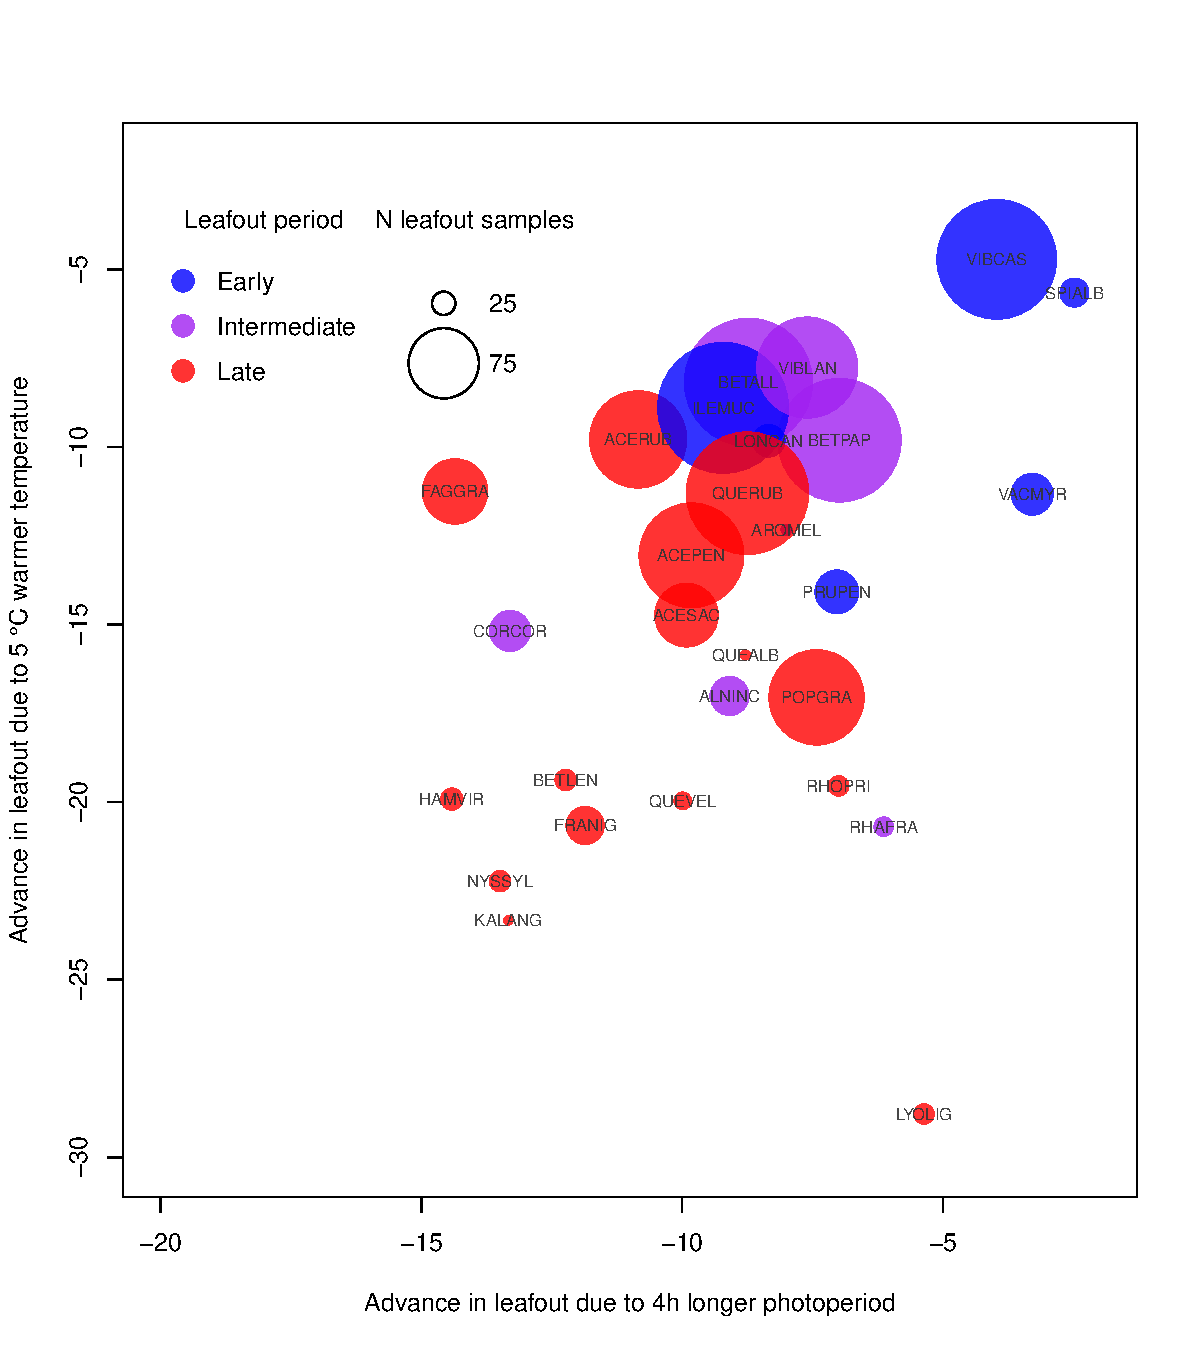
\includegraphics[scale=0.5]{Advplot2}
\label{fig1}
\end{center}
\end{figure}

% 2. model output
\begin{figure}
\begin{center}
\caption{Modeled effects plots, Budburst and leaf out}
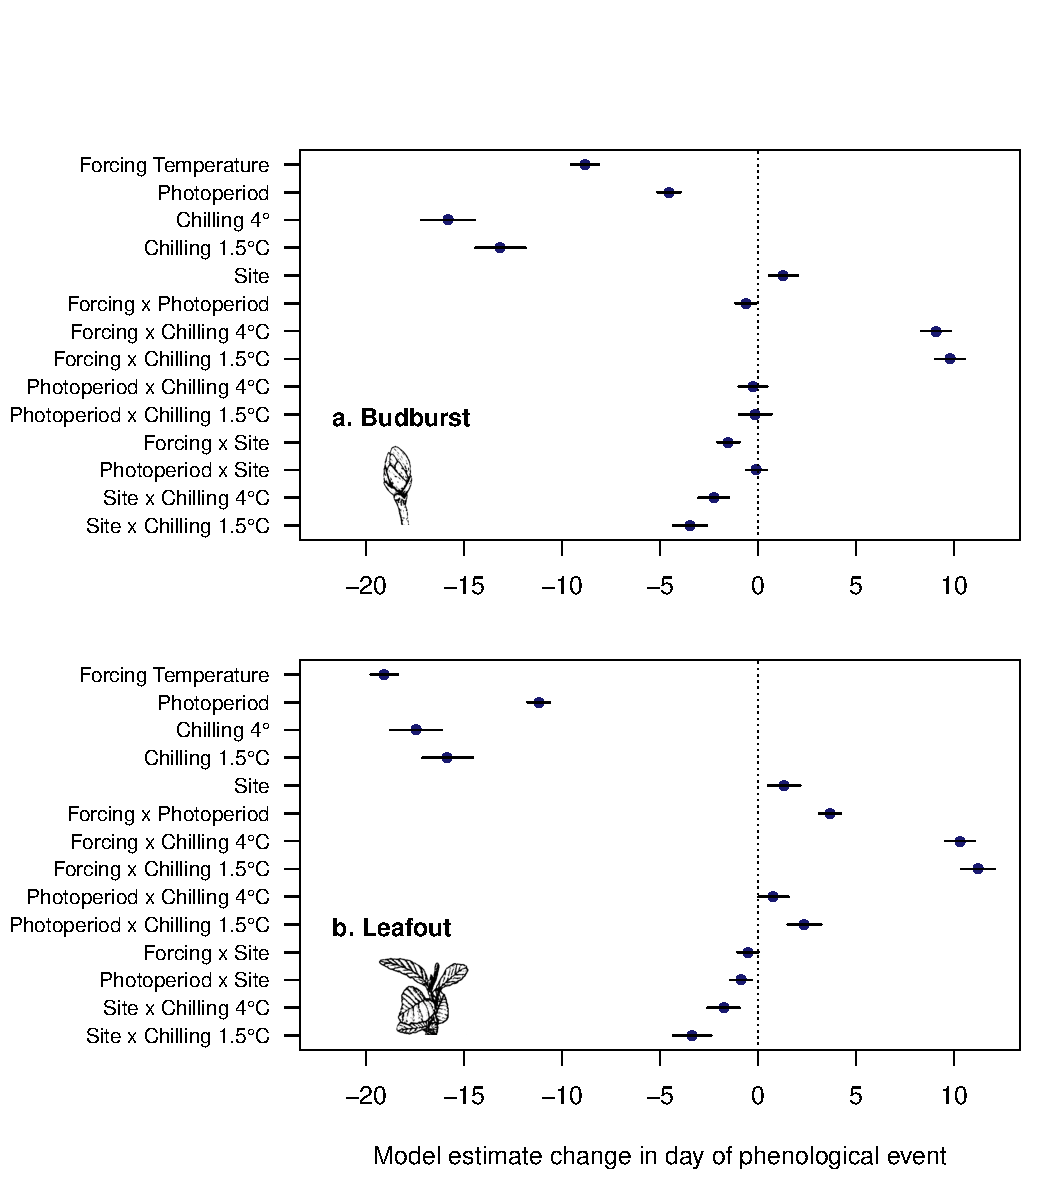
\includegraphics[scale=0.8]{Fig1_bb_lo}
\label{fig2}
\end{center}
\end{figure}

% 3. Temp + Pheno + Chill sensitivity

\begin{figure}
\caption{Sensitivity of budburst and leaf out to warming, leaf out, and chilling.}
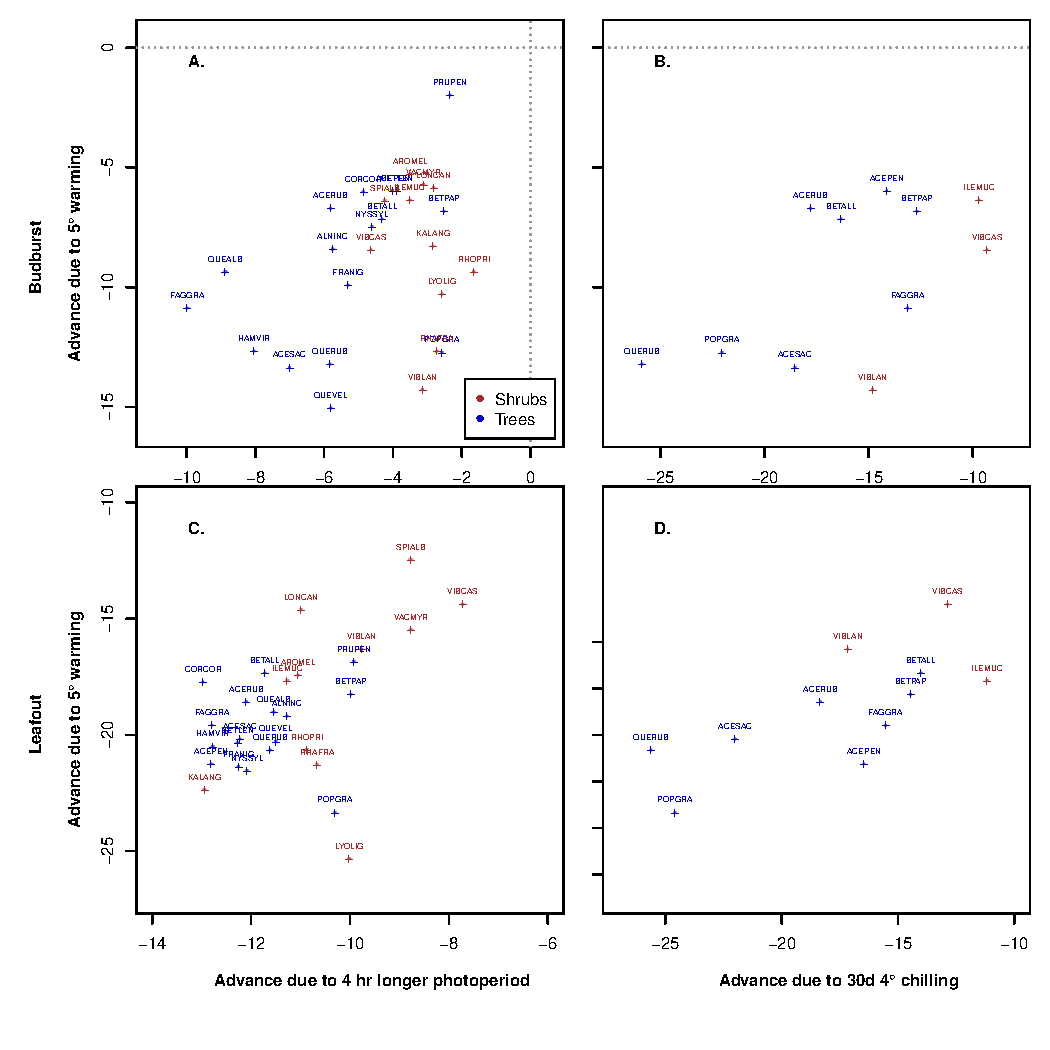
\includegraphics[scale=0.9]{Fig2_4panel}
\label{fig3}
\end{figure}

\end{document}}
